\documentclass[11pt,a4paper]{article}
\usepackage[margin=19mm,top=20mm,bottom=20mm]{geometry}
\usepackage{amsmath,amssymb,graphicx,array,fancyhdr,lastpage,textcomp,fancyvrb}
\usepackage{fontspec}
\usepackage[hidelinks]{hyperref}
\setmainfont{texgyreheros-regular.otf}[BoldFont=texgyreheros-bold.otf,ItalicFont=texgyreheros-italic.otf,BoldItalicFont=texgyreheros-bolditalic.otf]
\setmonofont{lmmono10-regular.otf}
\setlength{\parindent}{0pt}\setlength{\parskip}{5pt}
\setlength{\headheight}{14pt}
\pagestyle{fancy}\fancyhf{}
\renewcommand{\headrulewidth}{0.3pt}\renewcommand{\footrulewidth}{0.3pt}
\fancyfoot[L]{\footnotesize by paper.shrit.in\quad |\quad normal}
\fancyfoot[R]{\footnotesize Page \thepage\ of \pageref{LastPage}}
\begin{document}
\fancyhead[L]{\small Data Communication and Computer Networks}\fancyhead[R]{\small Set A: Ensemble}
{\LARGE\bfseries Worked Solutions}\par{\large Data Communication and Computer Networks}\par\textbf{Set A: Ensemble | CSE Semester 3}\par
Companion to \texttt{dccn-ensemble.pdf}. Question numbers match that paper. Equivalent correct methods are acceptable. These are independent worked solutions, not an official university marking scheme.\par\medskip\hrule\medskip
Questions 1--5: MCQ answer key, 1 mark each (5 marks total). Questions 6 onward: theory solutions (25 marks total).\par
\noindent\begin{minipage}{\linewidth}\subsection*{1. Layered headers}
\textbf{Correct option: (B).} The total is $900+5(20)=1000$ bytes.
\end{minipage}\par\medskip
\noindent\begin{minipage}{\linewidth}\subsection*{2. Header percentage}
\textbf{Correct option: (D).} The fraction is $100/(900+100)=0.10=10\%$.
\end{minipage}\par\medskip
\noindent\begin{minipage}{\linewidth}\subsection*{3. CRC degree}
\textbf{Correct option: (C).} The leading term is $x^4$, so the generator has degree 4.
\end{minipage}\par\medskip
\noindent\begin{minipage}{\linewidth}\subsection*{4. CRC appended zeros}
\textbf{Correct option: (A).} Append as many zeros as the generator degree, which is 4.
\end{minipage}\par\medskip
\noindent\begin{minipage}{\linewidth}\subsection*{5. Modulo-2 subtraction}
\textbf{Correct option: (B).} Modulo-2 subtraction is XOR, with no carry or borrow.
\end{minipage}\par\medskip
\noindent\begin{minipage}{\linewidth}\subsection*{6. ASK, FSK and PSK}

ASK changes carrier amplitude, FSK changes carrier frequency, and PSK changes carrier phase. Binary FSK commonly uses two separated frequencies and needs more bandwidth than binary PSK under comparable simple pulse shaping. ASK and BPSK can have comparable nominal bandwidth for the same bit rate and shaping; exact occupied bandwidth depends on the implementation. ASK is directly vulnerable to amplitude disturbances. Constant-envelope FSK and PSK are less affected by such disturbances, although phase/frequency noise and receiver synchronization still matter.

For a coherent receiver in an approximately additive-noise, bandwidth-limited telephone channel, BPSK is a defensible choice: it uses antipodal signals, offers good bit-error performance at a given energy per bit, and avoids the tone separation of binary FSK. A noncoherent, very simple receiver could instead favor FSK. The noise model and implementation must be stated rather than claiming one scheme is always best.
\end{minipage}\par\medskip
\noindent\begin{minipage}{\linewidth}\subsection*{7. Data rate and bandwidth}

Data rate is information bits transmitted per second. Here bandwidth means the span from the lowest to highest retained frequency. The three frequencies are 2, 6 and 10 MHz.
\[R_b=2f_0=2(2\ \mathrm{MHz})=\boxed{4\ \mathrm{Mbps}},\quad
B=10-2=\boxed{8\ \mathrm{MHz}}.\]
After tripling all frequencies, the components are 6, 18 and 30 MHz:
\[R_b'=\boxed{12\ \mathrm{Mbps}},\qquad B'=\boxed{24\ \mathrm{MHz}}.\]
For this fixed waveform model, both increase by a factor of three. A greater usable channel bandwidth permits faster signal changes, but achievable reliable data rate also depends on noise, signal levels and coding. The two-bits-per-cycle assumption is essential; it is not inferred from a sinusoid alone.
\end{minipage}\par\medskip
\noindent\begin{minipage}{\linewidth}\subsection*{8. Differential Manchester and AMI}

Start at a negative level. For differential Manchester, a 0 causes a transition at the start of its bit, a 1 does not, and every bit has a mid-bit transition. For AMI, zeros have zero level and successive ones alternate positive and negative, starting positive because the prior nonzero pulse was negative. The diagram labels each bit boundary.
\begin{center}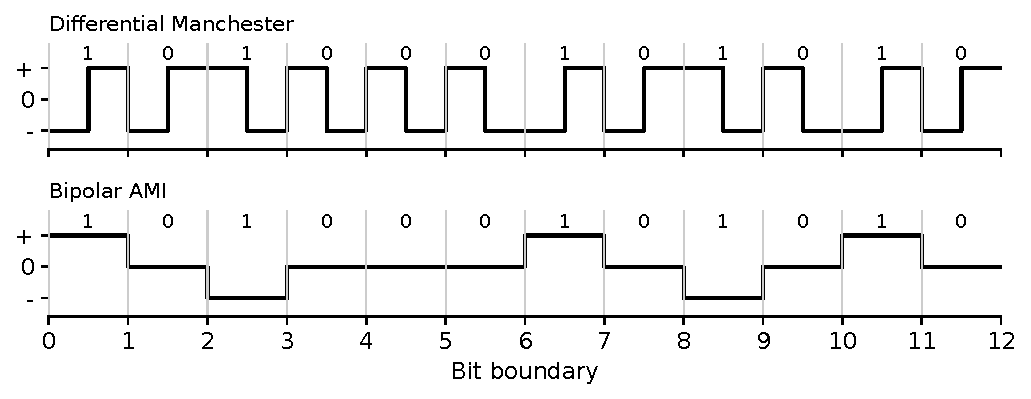
\includegraphics[width=.85\linewidth]{figures/line-source-3.pdf}\end{center}
\end{minipage}\par\medskip
\noindent\begin{minipage}{\linewidth}\subsection*{9. Manchester and AMI}

Use low-to-high for Manchester 1 and high-to-low for Manchester 0. AMI ones alternate polarity, with the first one positive; zeros are at zero level.
\begin{center}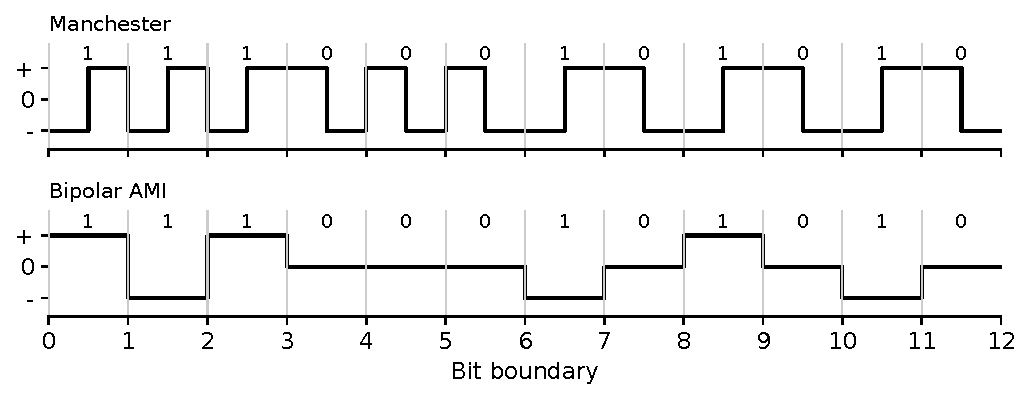
\includegraphics[width=.85\linewidth]{figures/line-source-4.pdf}\end{center}
\end{minipage}\par\medskip
\noindent\begin{minipage}{\linewidth}\subsection*{10. Hub, switch and router}

The hub repeats the Sales signal out its other ports without inspecting a destination address. HR and the attached switch therefore see it. The switch learns the source MAC address on the ingress port and forwards the frame only to the known IT destination port. If that MAC is unknown, it floods within the VLAN except back to the ingress port. A destination learned on the ingress port is filtered.

If Sales and IT are in the same IP subnet and VLAN, their local traffic need not pass through the Internet router. If they are in different subnets/VLANs, the sender uses its default gateway and the router must route between those networks. A router forwards according to destination IP and installs a new link-layer header on the outgoing link. Merely being connected to the Internet does not make it part of every local transfer.
\end{minipage}\par\medskip
\noindent\begin{minipage}{\linewidth}\subsection*{11. ARQ retransmission counts}

Initially frames 0, 1 and 2 are transmitted, with frame 1 lost.
\begin{center}\renewcommand{\arraystretch}{1.2}\begin{tabular}{lllll}\hline Protocol & Receiver handling of 2 & Retransmitted & Total sends & Useful/total\\\hline
Go-back-N & Discard & 1, 2 & 5 & 3/5 = 0.60\\
Selective repeat & Buffer & 1 & 4 & 3/4 = 0.75\\\hline\end{tabular}\end{center}Go-back-N has already accepted frame 0; on timeout it resends the outstanding suffix 1 and 2. Selective repeat acknowledges and buffers frame 2, then needs only frame 1 before delivering 1 and 2 in order. Counts use the clarified three-frame scenario printed in this paper, not the older ambiguous repeated-loss wording.
\end{minipage}\par\medskip
\noindent\begin{minipage}{\linewidth}\subsection*{12. Propagation-limited stop-and-wait time}

Number of frames $=10^6/2000=500$.
\[t_p=\frac{5000\times10^3}{2\times10^8}=0.025\ \mathrm{s},\quad
RTT=0.05\ \mathrm{s}.\]
Counting one complete round trip for each frame, including the final ACK, gives
\[T=500(0.05)=\boxed{25\ \mathrm{s}}.\]
Transmission, ACK serialization and processing times are neglected as requested.
\end{minipage}\par\medskip
\noindent\begin{minipage}{\linewidth}\subsection*{13. Collision-detection frame length}

\[t_p=\frac{1500}{3\times10^8}=5\ \mu\mathrm{s},\qquad
L_{\min}=R(2t_p)=10^8(10\times10^{-6})=\boxed{1000\ \mathrm{bits}}.\]
This is 125 bytes under the question's propagation-only model. The sender must still be transmitting when a far-end collision can propagate back.
\end{minipage}\par\medskip

\end{document}
